
\begin{slide}{XANES:  X-ray Absorption Near-Edge Spectroscopy}
\begin{cenpage}{120mm}
 Within $\sim$100eV of the absorption edge, the X-ray Absorption Spectra is
 highly sensitive to the chemical state and formal valence of absorbing element:
\end{cenpage}

\begin{cenpage}{150mm}
  \vmm
  \begin{columns}
    \begin{column}{48mm}
      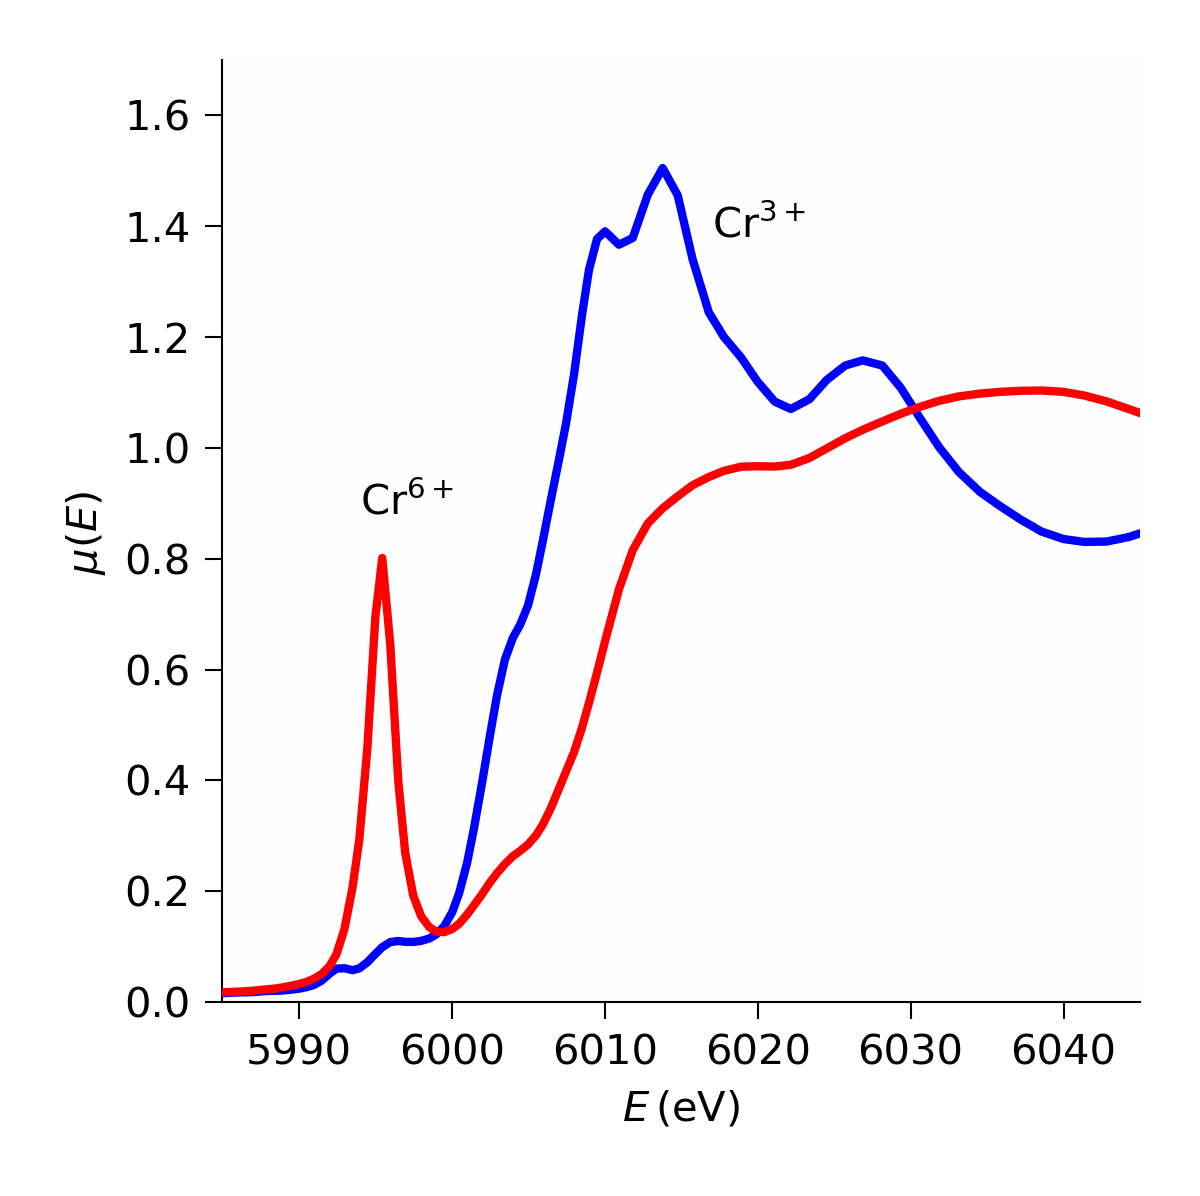
\includegraphics[width=48mm]{figs/xanes/cr}

      \vmm
      \hspace{5mm}  $\rm Cr^{3+}$ and $\rm Cr^{6+}$
    \end{column}
    \begin{column}{48mm}    
      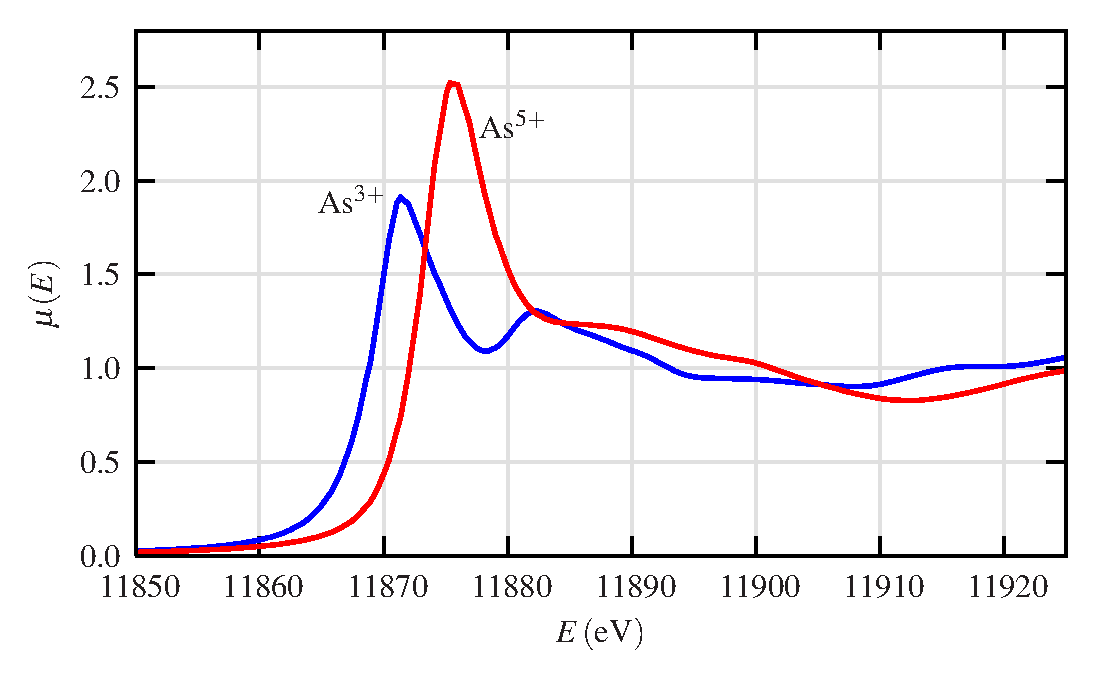
\includegraphics[width=48mm]{figs/xanes/as}
      
      \vmm
      \hspace{5mm}    $\rm As^{3+}$ and $\rm As^{5+}$
    \end{column}

    \begin{column}{48mm}
     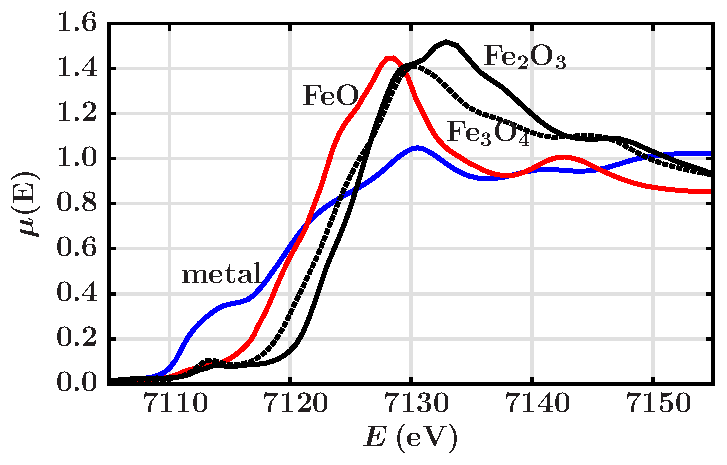
\includegraphics[width=48mm]{figs/xanes/fe_oxides}
      \hspace{5mm}    Fe metal and oxides.
    \end{column}
  \end{columns}

  \vmm
  
    The oxidation state and local atomic coordination environment strongly
    affect the lowest unfilled electronic levels of an absorbing atom.

    \vmm
    \begin{center}
      
    \begin{postitbox}{105mm}
        {\BlueEmph{what are the unoccupied electronic states
            that the photo-electron can fill?}}
    \end{postitbox}
  \end{center}

  \end{cenpage}

\vfill
\end{slide}

